%\begin{ccHtmlOnly}
%<center>
%<img border=0 src="./saarhull.gif" align=middle>
%</center>
%\end{ccHtmlOnly} 
%
%\begin{ccTexOnly}
%\begin{center}
%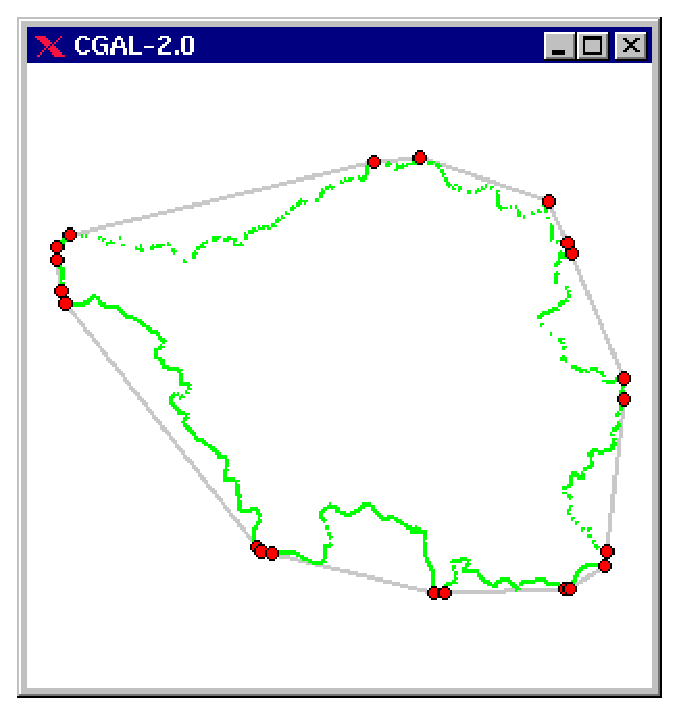
\includegraphics[width=6.5cm]{Convex_hull_2/saarhull}
%%\leavevmode\epsfxsize8cm\epsffile{Convex_hull_2/saarhull.eps}
%\end{center}
%\end{ccTexOnly}

\section{Spatial Sorting\label{sec:spatial_sorting}}

\cgal\ provides a small set of sorting algorithms, currently implemented only for 2D and 3D points, although it is easy to extend them to other objects through a traits mechanism.

Given an iterator range of points, the function \ccc{hilbert_sort} sorts them
along the space-filling Hilbert curve.
Combined with a \ccc{std::random_shuffle}, the function \ccc{spatial_sort} will
sort points in a way keeping enough randomness to retain theoretical optimality
for some algorithms\footnote{in fact, this has only been proved for Delaunay triangulation},
and close enough to a space-filling curve to speed-up algorithms.

The 2D and 3D triangulation classes of \cgal\ internally sort points as described
above, when the points are passed as an iterator range to a constructor or the
\ccc{insert} method.


% file currently missing
%\ccIncludeExampleCode{Spatial_sorting/sort_for_delaunay_2.cpp}


